\chapter{Fundamentals}

In this section, i am going to give a brief introduction about technologies and terminologies that are applied in this paper. 

\section{OPC Unified Architecture Structure Overview }
Object Linking and Embedding for Process Control Unified Architecture, known as OPC UA is the most recent released industry standards from OPC Foundation, acts nowadays as the most promising candidate in industry M2M automation world, whose major duty is to build a secure communication interface for machines that participate in automation system. 

\subsection{OPC UA Specifications}

The whole OPC Unified Architecture specification can be divided into three main parts:
\begin{itemize}
\item core specification part, which consists of OPC UA concepts, security model, address space model, services, information model, service mapping and profiles
\item access type specification part including data access, alarm and conditions, programs and historical access
\item utility specification part covering discovery together with aggregates.
\end{itemize}
\begin{table}[!htbp]
\caption{OPC UA specifications}
\centering
\begin{tabular}{lllll}
\hline\hline
OPC UA Part1 &Overview and Concepts Specification \\
OPC UA Part2 &Security Model Specification \\
OPC UA Part3 &Address Space Model Specification\\
OPC UA Part4 &Services Specification\\
OPC UA Part5 &Information Model Specification  \\
OPC UA Part6 &Mappings Specification \\
OPC UA Part7 &Profiles Specification \\
OPC UA Part8 &Data Access Specification  \\
OPC UA Part9 &Alarms and Conditions Specification \\
OPC UA Part10 &Programs Specification  \\
OPC UA Part11 &Historical Access Specification \\
OPC UA Part12 &Discovery and Aggregates Specification \\
\hline
\end{tabular}
\label{table:opcua}
\end{table}

\subsection{OPC UA Client Server Structure}
OPC UA standards apply the classic client server architecture, where server is in charge of managing functionalities provided by a machine as well as data information gathered by that device. Examples of sever functions could be reporting and monitoring temperature data measured by  a remotely allocated sensor and the make coffee function offered by a coffee maker. Meanwhile client possesses the ability to query information from server, submit subscription and send command to server.

\begin{figure}[!htbp]
	\centering
	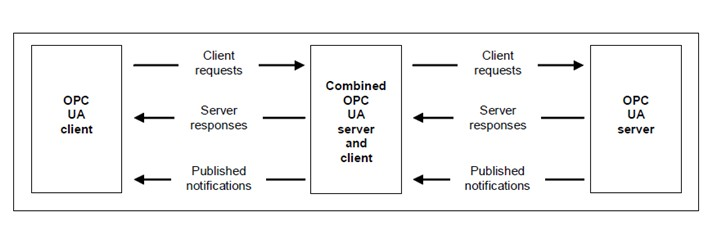
\includegraphics[width=1.00\textwidth]{cs.jpg}
		\caption{OPC UA Client Server Structure\cite{O1}}
	\label{fig:cs}
\end{figure}
Figure~\ref{fig:cs} illustrates a typical OPC UA client server architecture and also describes an internal combined server-client structure. The routine communication between client and server consists of requests from client, corresponding responses sent by server and notifications which are generated because of client's early subscription.

\subsection{OPC UA Terminologies}
In OPC Unified Architecture on server stored information that can be visited by clients is defined as \emph{address space}\cite{O3} and there also exits a set of services\cite{O4} which are provided by server and are introduced in order to apply operations on \emph{address space}. Information in address space is organized as a set of in particular hierarchy structured \emph{Objects}. \emph{Object} here could refer to data gathered by sensor, server system parameters and etc. Clients can query and accept information provided by OPC Unified Architecture Servers in two major ways, \emph{binary structured data} and \emph{XML documents}, depending on the complexity of exchanged data, network quality and so on. In addition three kinds of transport protocol are already defined to support client server communication. They are: \emph{OPC UA TCP}, \emph{HTTP/SOAP} and \emph{HTTP}. Also the hierarchy structure in which \emph{Objects} are organized in \emph{address space} is also various and not only limited to simple single hierarchy.   

One of the charming features provided by OPC UA is \emph{Event Notifications}. With the help of \emph{Event Notification}, OPC UA servers are allowed immediately after satisfaction of conditions, which is normally predefined by a client, to publish data to particular client. In this way, clients can for instance discovery failures within client-server-communication quickly and recover that communication as soon as possible, which in return minimizes the lost to the smallest possible amount. Also clients are able to observe the subscribed data more precisely and find the pink elephant as fast as possible.

\subsection{Standard OPC UA Server}
\begin{figure}[!htbp]
	\centering
	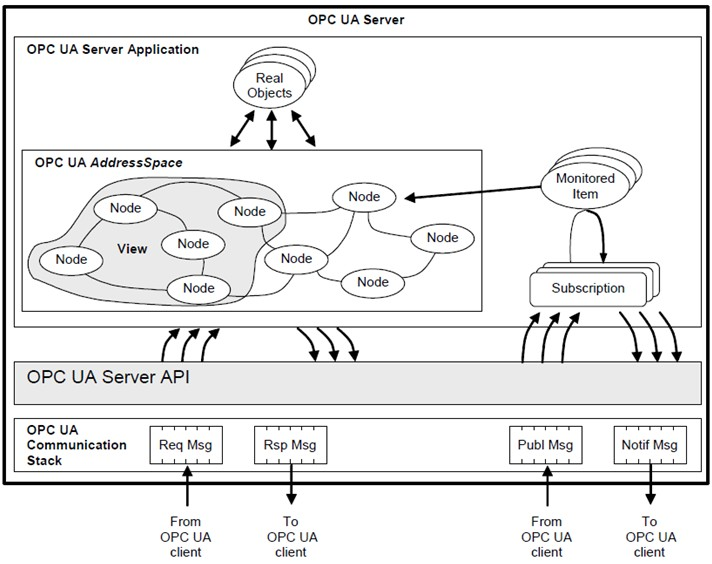
\includegraphics[width=0.8\textwidth]{server.jpg}
		\caption{OPC UA Server Structure\cite{O1}}
	\label{fig:server}
\end{figure}
In figure~\ref{fig:server}, the structure of one standard OPC UA Server is described. It includes three main parts, server application, internal API and communication stack. In server application part,  functionalities and services which are offered by OPC UA standards are realized, such as \emph{Event Notification} , processing request from connected OPC UA client, data encryption and decryption. Moreover, \emph{Real objects}  here  refers physical field devices and software applications that are maintained and managed by OPC UA server. \emph{Nodes} in \emph{Address Space} presents  abstractly above mentioned \emph{Real Ojbects}. \emph{View}, which is pictured as a part of address space, presents \emph{Objects} that can be browsed by particular clients. The main  task for communication stack  is to establish communication session based on secure channel between OPC UA client and server. Typically communication messages which are exchanged frequently among clients and servers are, request-, notification- message from client and   corresponding   response-, publish message from server. At last, an internal API connects the server application and the communication stack.

\subsection{Standard OPC UA Client}
\begin{figure}[!htbp]
	\centering
	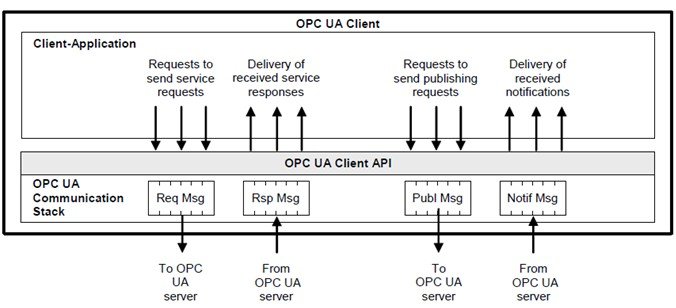
\includegraphics[width=1.0\textwidth]{client.jpg}
		\caption{OPC UA Client Structure\cite{O1}}
	\label{fig:client}
\end{figure}

Figure~\ref{fig:client} pictures one simple OPC UA client containing client application, an internal API, isolating the application code from communication stack, and a communication stack that converts API calls into messages and delivers them to OPC UA server.

\subsection{Secure Channel and Session}

\begin{figure}[!htbp]
	\centering
	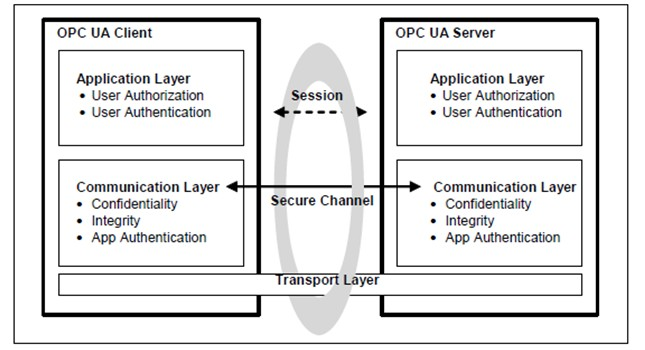
\includegraphics[width=0.8\textwidth]{opc_ua_cs_comm.jpg}
		\caption{OPC UA Client Server Communication\cite{O2}}
	\label{fig:opc_ua_cs_comm}
\end{figure}

Since some data exchanged between client and server could be extreme precious and should be protected from other malicious third party, OPC UA defines a full set of  \emph{security model}, with which sytem developer can configure the security level of the application to meet the need of reality. In the \emph{security model}, authentication of client and server, authorization, integrity and confidentiality of client-server-communication, auditability(also known as traceability ) and availability of services are guaranteed. Also OPC UA  standard provides a set of countermeasures against attacks such as message flooding, eavesdropping, message spoofing, message alteration, message reply, server profiling, session hijacking and so on\cite{O2}.


Figure~\ref{fig:opc_ua_cs_comm} pictures the typical communication architecture between OPC UA client and server. As shown in~\ref{fig:opc_ua_cs_comm}, the communication between OPC UA client and server is established above a secure channel, which is active during the whole application session and in this session, the state information, such as algorithms used for authentication, user credentials, is maintained. The secure channel is established only after successful validation of both client and server certificates and it provides necessary mechanisms to support confidentiality, message integrity and application authentication. On top of secure channel, is an application level session between OPC UA client and server, whose responsibility is to transmit data information and commands. It should be pointed out that, even a secure channel is out of work for some reasons, the session is still valid and OPC UA client and server involved in aforementioned session can still re-establish the broken secure channel. A secure transport layer is guaranteed by encryption and signatures methods provided by platform that supports OPC UA structure.

\begin{figure}[!htbp]
	\centering
	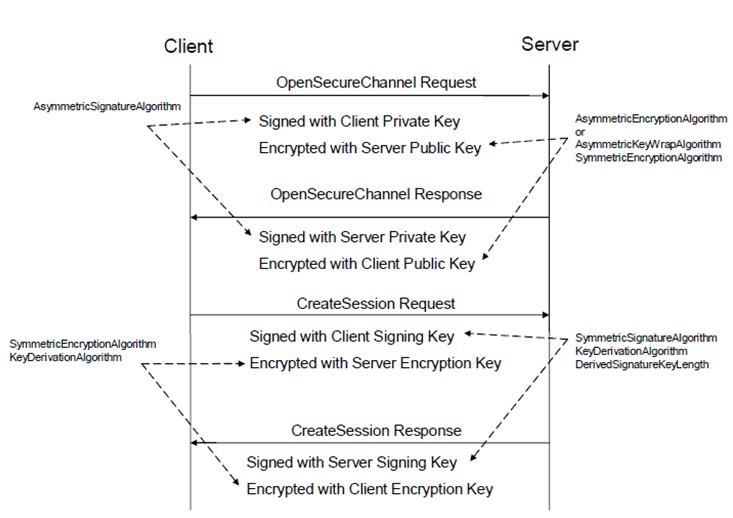
\includegraphics[width=0.7\textwidth]{opc_ua_shs.jpg}
		\caption{OPC UA Client Server Security Handshake\cite{O2}}
	\label{fig:opc_ua_cs_shs}
\end{figure}

\subsection{Security Handshake}
Security handshake as below explains with some details how secure channel and session are established. Normally OPC UA client initiates the first \emph{OpenSecureChannel} request and waits the response from server. Messages exchanged during the process of construction secure channel between client and server are encrypted using asymmetric encryption and signature algorithms. But some security protocols that could be applied according to OPC UA standards, are not using an asymmetric message encryption algorithm to encrypt to request/response messages. Instead, they apply AsymmetricKeyWrapAlgorithm to encrypt symmetric keys and use symmetric encryption algorithm with encrypted keys to encrypt messages. After a successful construction of secure channel, OPC UA client sends \emph{CreateSession} request and waits for server response. Messages transported during this procedure are encrypted with symmetric encryption algorithms and signed with client/server signing key.
\begin{figure}[!htbp]
	\centering
	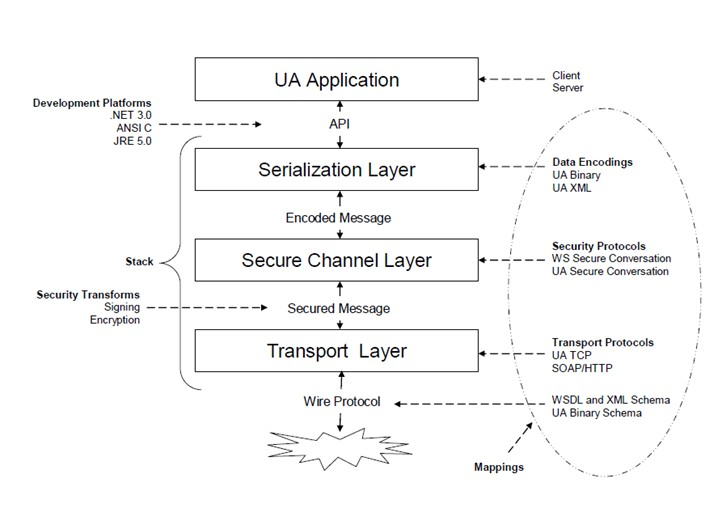
\includegraphics[width=0.7\textwidth]{opc_ua_commstack.jpg}
		\caption{OPC UA Client Server Communication Stack\cite{O2}}
	\label{fig:opc_ua_commstack}
\end{figure}

\subsection{OPC UA Communication stack}
As described in figure~\ref{fig:opc_ua_commstack}, according to different responsibility, OPC UA communication stack consists of three parts: application layer, communication layer and transport layer. Even the terminologies of those layers using the same English words as the ones used in ISO model, but they are not equal to layers in ISO model. Figure~\ref{fig:opc_ua_commstack} also pictures a precise functionality overview of each component.

UA Application part realizes client or server application. Serialization layer together with secure channel layer build the communication layer and their job is dividing long message into pieces referred as message chunk, encrypting each individual message chunk and forwarding encrypted message chunk to transport layer. When receiving message chunk from others, OPC UA message receiver firstly verifies whether this message piece meets the security standard negotiated between OPC UA client and server. If not, message receiver will close the secure channel. After a successful verification of all message chunks, the original OPC UA message will be reconstructed and sent to UA Application Code through API. Each secure message chunk applies the following structure described in figure~\ref{fig:opc_ua_messchunk}.

\subsection{Other Competitor}
WebSphere Message Broker Message Queuing Telemetry Transport (MQTT)\cite{Ref3} is another machine to machine (M2M) communication protocol. Compared with OPC UA standard, MQTT also supports UDP protocol in the transport layer. In OPC UA, only unidirectional, client to server, communication is provided, but in MQTT server to client communication is also possible without server implements client code. Moreover the communication overhead of MQTT is in comparison with OPC UA is relative small. 


Even thought MQTT protocol supports communication environment with low bandwidth and high latency, OPC UA provides complex object model and supports more features, including historical data record, alarm, notification, complete security policies and this is reason why OPC UA is more suitable for the application scenario that handles sensitive data with complex structure and needs immediate response.


Another member from Internet of Things is Constrained Application Protocol (CoAP)\cite{Ref5} which is designed for the extreme simple electronic devices with less memory and computing power and original CoAP only runs over UDP. Compared with OPC UA, simplicity from CoAP is the advantage, but apparently it should be considered that in the implementation scenario other transport protocol could be used, like TCP, more functions and services other than pure message exchange between client and server, are requested from users.

\section{Smart card}
\subsection{Overview}
Smart Card, whose characteristic feature is an integrated circuit that is embedded in a chip card, which is capable of performing data process, information storage and message transmitting\cite{handbuch}. The most charming feature of smart card is that, sensitive user's credential data such as certificates, encryption keys, digital signature along with other precious user information can only be accessed though a serial interface, which stands under  strict control of the card operation system. This characteristic provides strong  protection against  unauthorized data access and ensures the confidentiality of on card stored information. Therefor smart cards are widely used in applications that require strong protection.

With sophisticated communication protocol using Application Protocol Data Units(APDU), smart card and Card Accepting Device(CAD) are able to process secure message exchange. Smart card is also able to process cryptographic algorithms on hardware. Nowadays, it supports symmetric key algorithms like DES, triple DES; standard public key cryptography for instance RSA, hash functions such as commonly SHA-1\cite{handbuch}. More powerful microprocessor on chip card is, the speed performance is better.  

\begin{table}[ht]
\caption{ISO/IEC 7816\cite{handbuch}}
\centering
\begin{tabular}{lllll}
 ISO7816 document & Description  \\[1ex]
\hline\hline
 ISO 7816-1&Physical characteristics   \\
ISO 7816-2&Dimensions and location of the contacts   \\
 ISO 7816-3& Electronic signals and transmission protocols   \\
ISO 7816-4&Industry commands for interchange  \\
ISO 7816-5& Number system and registration procedure for application identifiers \\
ISO 7816-6& Interindustry data elements  \\
\hline
\end{tabular}
\label{table:ISO7816}
\end{table}

In ISO/IEC 7816 standards family,  the smart card's fundamental properties and functionalities are defined.

\begin{figure}[!htbp]
	\centering
	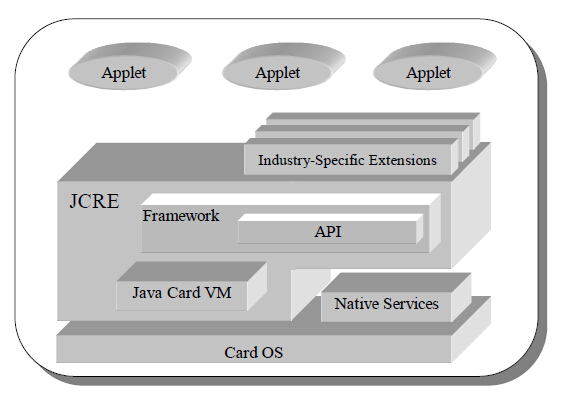
\includegraphics[width=0.8\textwidth]{scc.jpg}
		\caption{Smart Card Software Components\cite{jcadg}}
	\label{fig:scc}
\end{figure}

\subsection{Universal integrated Circuit Card}
The Universal Integrated Circuit Card is the smart card used in mobile terminals in GSM and UMTS networks. It enables authenticated subscriber to join the network with their mobile terminals and at the same time protects essential user data. UICC acts  also most time as the secure token, which stores and protects subscriber's confidential information. Moreover, as a 32bit processor, UICC is also capable of processing necessary  encryption and  decryption algorithms\cite{uiccDef}.

\subsection{Smart Card Software Components}
As illustrated in figure~\ref{fig:scc}, one typical smart card software includes Card Operation System, native services such as I/O operation and memory management, Java Card Runtime Environment(JCRE) that consists of Java card  Virtual Machine and Framework who is in charge of dispatching APDU as well as applet management, installed applet and at last other optional industry specific extensions\cite{jcadg}

\subsection{Smart card File Management}
One of smart card's characteristics is data storage media. But in contrast with other storage device, the most distinguishing feature of smart card file system is that, there exists no man-machine interface\cite{handbuch}, which means all files are addressed with help of hexadecimal codes and every single file process command is strictly based on this shema.

\begin{figure}[!htbp]
	\centering
	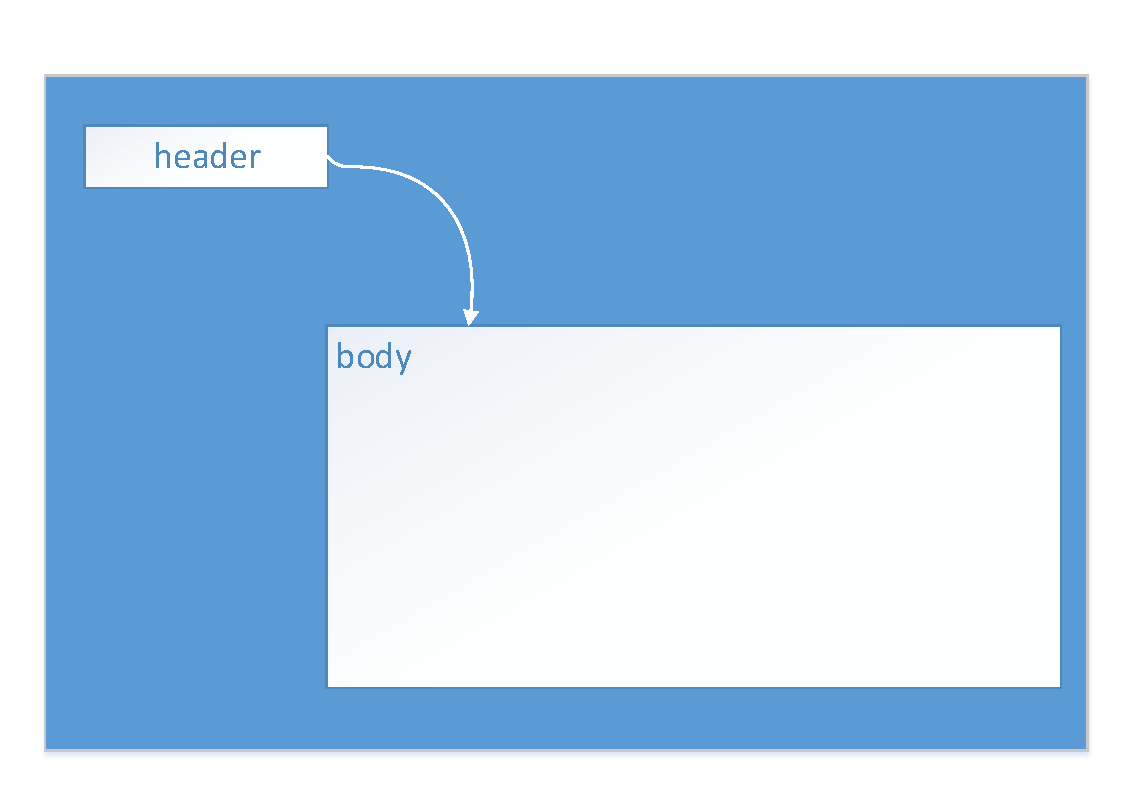
\includegraphics[width=0.8\textwidth]{file}
		\caption{the internal structure of a file in smart card file management system\cite{handbuch}}
	\label{fig:file}
\end{figure}

\subsubsection{File Structure}
As pictured in figure~\ref{fig:file}, files on smart card consist of two parts,  the header, which encapsulates administrative information such as, file structure and access conditions, the body, that stores real user data and is linked with file header using a pointer. This file management mechanism has its own advantage. To be more specifically, since file header and body are separately located, therefore even write/read error occurs in file body, file header, which is under normal circumstances never altered and saves essential access conditions, will not be affected, which in return provides better physical storage security.

\subsubsection{File Types}
According to ISO/IEC 7816-4 specification, smart card offers two major file types, dedicated file (DF) and elementary file (EF). DF is also described as directory file, which contains lower-level DFs and EFs. And in EF, real user data is stored. Moreover there is a special DF, called master file (MF), which represents root directory of smart card file system and only selected by smart card OS. Figure~\ref{fig:file-structure} illustrates one possible architecture of smart card file system.

\begin{figure}[!htbp]
	\centering
	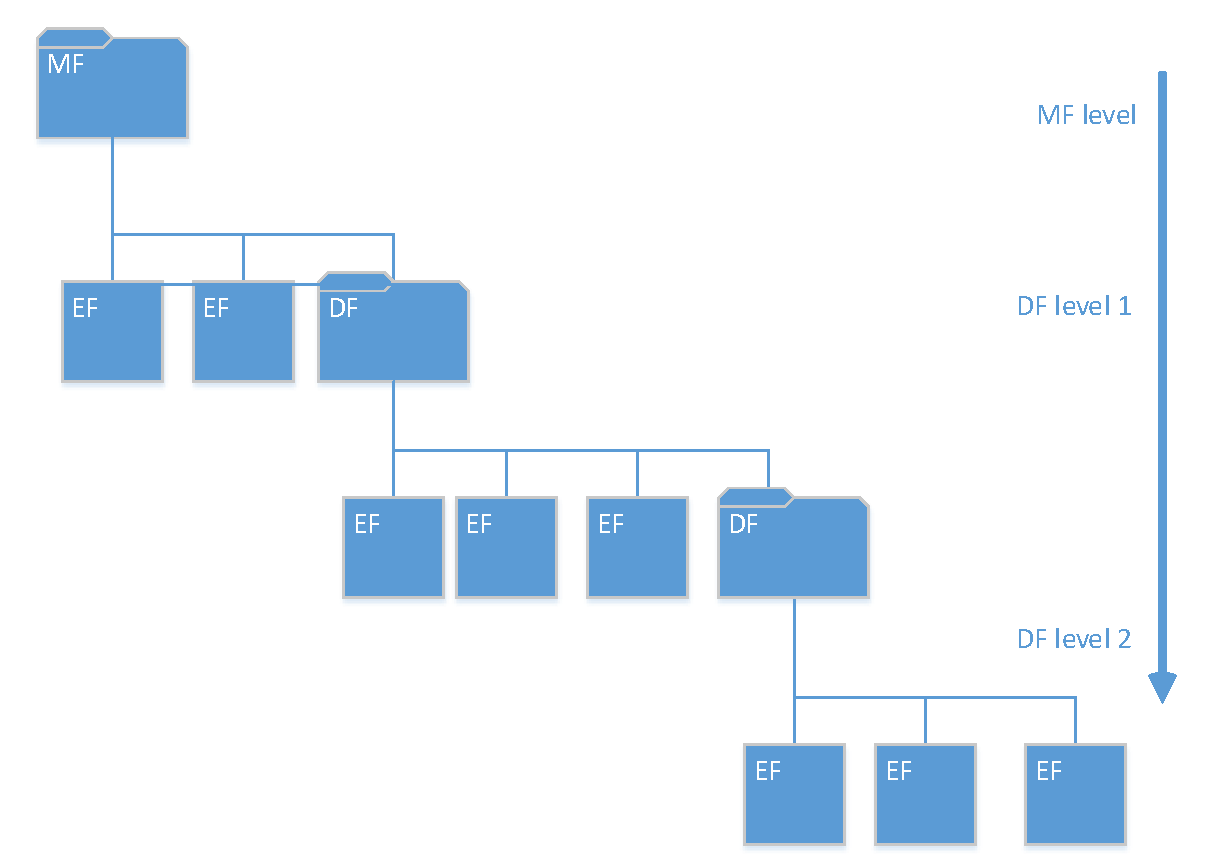
\includegraphics[width=0.7\textwidth]{file-structure}
		\caption{File Tree on Smart Card\cite{handbuch}}
	\label{fig:file-structure}
\end{figure}

\subsubsection{PKCS{\#}15}
As already shown, smart card not only is used as storage media but also acts as cryptographic token which offers enhanced security and privacy functionalities for other applications. The PKCS\#15 (Public key cryptography standards) specification\cite{pkcs}, which was proposed by RSA Inc. and is nowadays worldwide accepted, provide standards, that define how to store credential information such as cryptographic keys, certificates on smart card, and how to retrieve specified token with help from PKCS\#15 interpreter.
 
\subsection{Data Exchange with Smart Card}

\begin{figure}[!htbp]
	\centering
	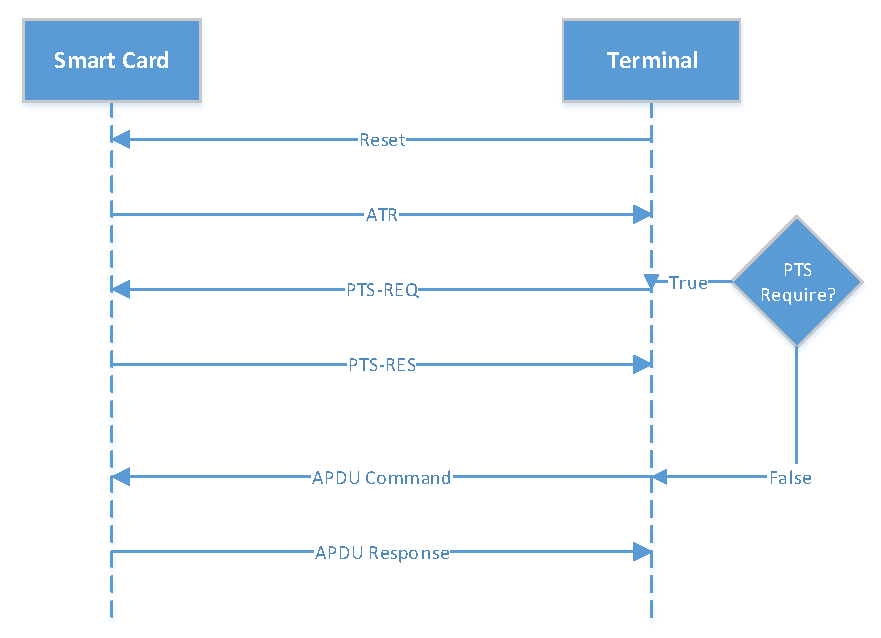
\includegraphics[width=0.7\textwidth]{master-slave-relationship}
		\caption{Communication between Smart card and CAD\cite{handbuch}}
	\label{fig:master-slave-relationship}
\end{figure}
The communication protocol between smart card and terminal is described as Master-Slave relationship\cite{handbuch}, that means terminal device knowns as Master processes unidirectional control over its slave, namely smart card. Once Master-Slave relationship is established, each communication will be initialized by Master and Slave only reacts based on Master's command. 

When a smart card is inserted in a terminal, Master will send its Slave a RESET command which causes smart card to perform a Power-on-Reset behavior. After this Power-on-Reset, smart card informs Master using Answer-to-Rest (ATR) message about card state and communication parameters. In the next step, if necessary terminal will generate a Protocol Type Select (PTS) command, which is used to choose communication protocol and parameters suggested by smart card. After a successful negotiation, smart card and terminal are able to exchange data using Application Protocol Data Unit.
  
Application Protocol Data Unit, or APDU for short, is used  to perform data exchange between smart card and CAD and its structures satisfy ISO 7816-4 specification\cite{chen}. There are two categories of APDU, namely command APDU and response APDU. Command APDU structure and response APDU structure are described in Table~\ref{table:capdu} and Table~\ref{table:rapdu} respectively\cite{handbuch}. 

\begin{table}[!htbp]
\caption{Command APDU Structure}
\centering
\begin{tabular}{lllll}
\hline\hline
 CLA &class byte identifying application  & mandatory \\[0.5ex]
 INS &instruction byte representing the actual command  & mandatory \\
 P1 &parameter 1 used to provide more command information & mandatory \\
 P2 &parameter 2 used to provide more command information& mandatory \\
 Lc field &the length of data received by card & mandatory \\
 data field &data sent to card& optional \\
Le field &the length of data sent by card& optional \\
\hline
\end{tabular}
\label{table:capdu}
\end{table}

\begin{table}[ht]
\caption{Command APDU Structure}
\centering
\begin{tabular}{lllll}
\hline\hline
 data field & length decided by Le of preceding command  APDU  & mandatory \\[0.5ex]
 SW1 &state word 1 also called return code 1  & mandatory \\
 SW2 &state word 2 also called return code 2& mandatory \\
\hline
\end{tabular}
\label{table:rapdu}
\end{table}

\subsection{Secure Messaging}
Since all communication between smart card and terminal is based on digital electrical pulse performed on card I/O line, attacker can easily record all communication information and and recover it. Therefore secure messaging mechanism is proposed and used to protect against aforementioned message eavesdropping, to ensure authenticity and confidentiality of exchanged information.

In secure message mechanism, both message sender and receiver must agree on to be applied message cryptographic algorithms and corresponding pre-shared keys. In telecommunication domain in accordance with ISO/IEC 7816-4\cite{handbuch}, TLV(Type-lengthl-valuse)-formed data, which encapsulates relative user information, is used to perform secure messaging as data carrier.

\subsection{Life Cycle}
The typical Life cycle of a smart card is described as following\cite{smart_card_contactless}:
\begin{itemize}
\item \emph{Fabrication Phase} As the start of smart card life cycle, this process is taken by the card manufactures. One unique \emph{fabrication key}, \emph{KF} for short, is applied in order to keep smart card from unauthorized modification. 
\item \emph{Pre-personalization Phase} After fabrication phase,  smart card chip is gonging to be integrated on plastic frame by card suppliers. Moreover \emph{fabrication key}, which is derived from \emph{manufacturer key} in phase one, is replaced by a \emph{personalization key}, which is also known as \emph{KP},  for the purpose of secure smart card delivery to card issuer. In order to protect smart card from fraudulent changes, \emph{KP} is locked by a \emph{personalization lock}.
\item \emph{Personalization Phase} In this phase,  card issuer will write complete data files on the card including card PIN, card holder identity and so on. When card issuer finish this phase, he will add an \emph{utilization lock} and the life cycle of smart card will come to next phase.
\item \emph{Utilization Phase} Card holder will be able to use his smart card in this phase. But the information access still must follow the rules defined by to be visited applications.
\item \emph{Invalidation Phase} Card operation system will block the smart card in this phase. To be more specifically, operation such as writing and update will be disabled. There are two reasons that why a smart card lands this phase. Reason one is because both \emph{smart card PIN} and \emph{smart card unblock PIN} reach its limited  try counts, which indicates someone is trying to force brute guessing PIN.  The other reason is, a particular application adds a \emph{invalidation lock} on \emph{master file} of smart card.
\end{itemize}

\subsubsection {Conclusion}
From the above described smart card life cycle, it is not hard to find out that from the every begin of smart card manufacturing and deliver process, card manufacturers and issuers have taken it into account, that a secure card production, utilization and delivery must be guaranteed.

\section{Java Card}
Java Card technology not only adopts the distinguishing features from Java, such as productivity, security and portability\cite{jcadg}, it also makes Java technology available on smart card, where programmer must be faced with more harsh conditions, like limited memory resource and computer ability.

In contrast with Java VM, Java Card VM consists of two parts, the on-card part, which is in charge of bytecode execution, class as well as object management and secure data exchange, the off-card part, which is the real Java Converter.
 \begin{figure}[!htbp]
	\centering
	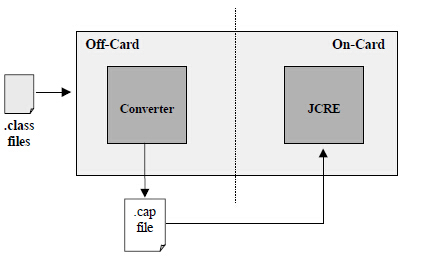
\includegraphics[width=1\textwidth]{jcvm.jpg}
		\caption{Java Card VM Components\cite{jcadg}}
	\label{fig:jcvm}
\end{figure}
As illustrated in figure~\ref{fig:jcvm}, a complied Java applet (.cap file) is generated by off-card Converter based on inputed Java class file and executed by on-card Java Card Runtime Environment (JCRE). 

\subsection{Language Specification}
Apart from above mentioned Java Card VM, compared with original Java language, Java card has many unique features.
Since current smart card does not support multitasking, therefore threads are not backed up in Java Card. Also garbage collection  is performed by VM, as a result function \emph{finalize()} is not supported. Moreover because on smart card, memory space and process ability is limited, as a result programmer can only use three main primitive types, namely byte, short and boolean. Furthermore only one-dimensional array is offered. Nonetheless Java card language supports all features of inheritance and provides all Java language security features, for example, private access modifiers as well as bytecode verification\cite{jcadg}.

\subsection{Transaction Integrity}
One of the most import features of Java Card technology is that Java Card Runtime Environment ensures the integrity of transaction, which means even an unexpected loss of power occurs on smart card, the ongoing transactions' integrity is protected with the help of following schema\cite{handbuch}:
\begin{verbatim}
// Transaction Starts
JCSystem.beginTranscation();

doSomething

//Transaction Ends
JCSystem.commitTransaction();
\end{verbatim}
Only when JCRE finishes running method \emph{JCSystem.commitTranscation()}, the corresponding transaction will be finished and submitted. Otherwise JCRE will throw transaction exception and reset data that involved in this broken transaction.

\subsection{Persistent Object and Transient Object}
In  the realm of Java Card, all objects are preserved in nonvolatile memory, which means this persistent object exits on smart card beyond the execution time of corresponding applet, as long as there exits a reference pointing to it. But also it is allowed to develop transient object on Java card. To be precisely, for instance class array object stays in nonvolatile memory space but in contrast one actual instance of array in stored in volatile memory\cite{handbuch}.

\subsection{Java Card Applet}
Java Card Applet refers to the Java Card language programmed code, which extends the class \emph{Applet} from package \emph{javacard.framework}. Meanwhile Java Card Applet should implement following four methods:
\begin{itemize}
\item\emph{install()}, this method must be implemented and be used to create an applet instance.
\item\emph{process(APDU)}, the implementation of this method is also mandatory and uses APDU as input parameter. In this method applet developer designs how to process APDU sent to this applet and which APDU response should be generated.
\item \emph{select()}, when JCRE detects a SELECT APDU command, which is applied to select one installed applet, JCRE will call this method of to be selected applet.
\item  \emph{deselect()}, this method is called by JCRE to inform corresponding applet that it is no longer selected by JCRE.
\end{itemize}

\begin{figure}[!htbp]
	\centering
	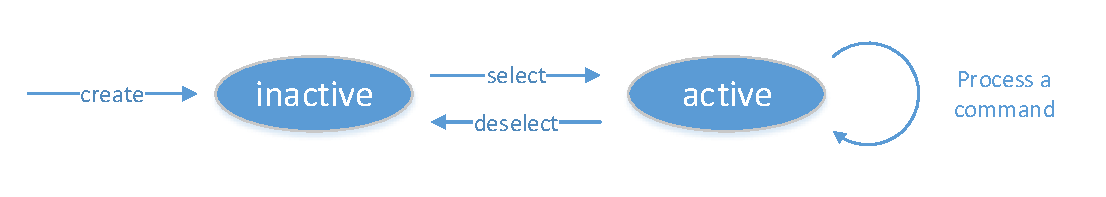
\includegraphics[width=1\textwidth]{applet-execution-states}
		\caption{Javacard Applet Execution States\cite{handbuch}}
	\label{fig:applet-execution-states}
\end{figure}
After finishing programming one Applet, it comes to next phase, namely applet installation. This process takes place usually at the factory or office under the control of card issuer. When one applet is installed on smart card, it only directly communicates with JCRE and other installed applet classes. It should be pointed out, this installed Java Card applet is also belongs to \emph{persistent object} and stored in smart card nonvolatile memory space. Every Java Card Applet is assigned one unique Application ID, which is also known as AID and be used by JCRE to \emph{register} and \emph{select} corresponding applet at run time.

Figure~\ref{fig:applet-execution-states} pictures execution states transaction of Javacard applet. Furthermore figure~\ref{fig:apdu-command-processing} illustrates how JCRE selects and deselects one applet based on input APDU commands.

\begin{figure}[!htbp]
	\centering
	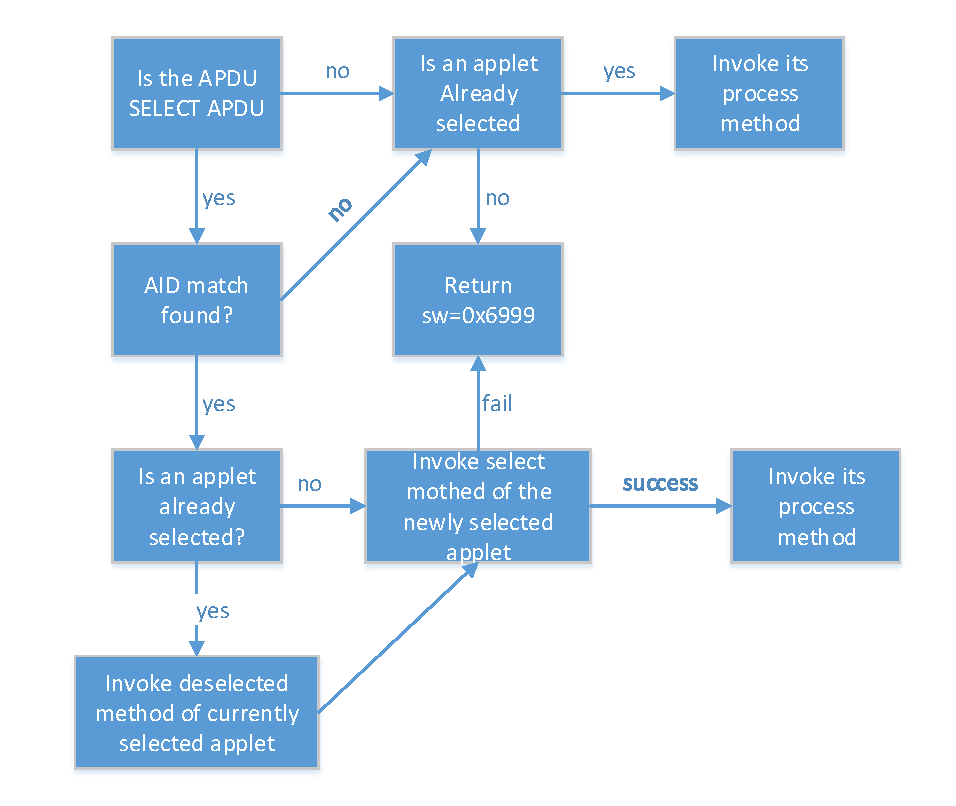
\includegraphics[width=0.8\textwidth]{apdu-command-processing}
		\caption{APDU command processing\cite{handbuch}}
	\label{fig:apdu-command-processing}
\end{figure}


\subsection{Javacard Cryptography}
Javacard provides a list of APIs to support not only smart card application and data exchange security but also to reinforce other system's security by acting as essential security token. 
In order to ensure sure messaging between smart card and terminal following three aspects must be considered:
\begin{itemize}
\item \emph{Entity Authentication:} Usually mutual authentication is applied to guarantee the authorities of both communication partners.
\item \emph{Message Confidentiality:} The transfered information is encrypted using algorithms negotiated between two communication entities to ensure data privacy and security.
\item \emph{Message Integrity:} In order to protect exchanged message from unauthorized modification and to provide authenticity assurance, message authentication code (MAC) is calculated based on to be transfered data and integrated in that message.
\end{itemize}
Packages \emph{javacard.security} and \emph{javacardx.crypto} support aforementioned security mechanism with following class and interfaces\cite{chen}:

\begin{table}[!htbp]
\caption{package:\emph{javacardx.crypto}}
\begin{tabular}{lllll}
\hline\hline
Class or Interface & Function Description\\[0.5ex]
Cipher & \parbox[t]{10cm}{Abstract class offers cryptographic cipher used for encryption and decryption}\\
KeyEncryption & Class provides implementation of keys\\
\hline
\end{tabular}
\label{table:javacardx-crypto}
\end{table}


\begin{table}[ht]
\caption{package: \emph{javacard.security}}
\centering
\begin{tabular}{lllll}
\hline
 Class or Interface & Function Description\\
\hline\hline
 Key &Interface for all keys   \\
 SecrectKey &Interface for symmetric algorithms' keys\\
DESKey & \parbox[t]{10cm}{Interface for keys used for DES or two-key triple DES or three-key triple DES}\\
PrivateKey &Interface for private keys\\
PublicKey & Interface for public keys\\
RSAPrivateKey& Interface for keys used by RSA algorithm to sign data\\
RSAPublicKey & Interface for keys used to verify signatures generated with RSA \\
DSAKey& Interface for keys used by DSA\\ 
DSAPrivateKey& Interface for keys to sign data with DSA algorithm\\
DSAPublicKey& Interface for keys to verify signatures generated with DSA\\
KeyBuilder& Factory class implemented to construct key objects\\
MessageDigest& Abstract class for hashing algorithm\\
Signature& Abstract class for signature algorithm\\
RandomData&Abstract class for generation of random data \\
CrptoException& Exception class\\
\hline
\end{tabular}
\label{table:javacard-security}
\end{table}


\section{GlobalPlatform and Remote Application Management}\label{secGP}

\begin{figure}[!htbp]
	\centering
	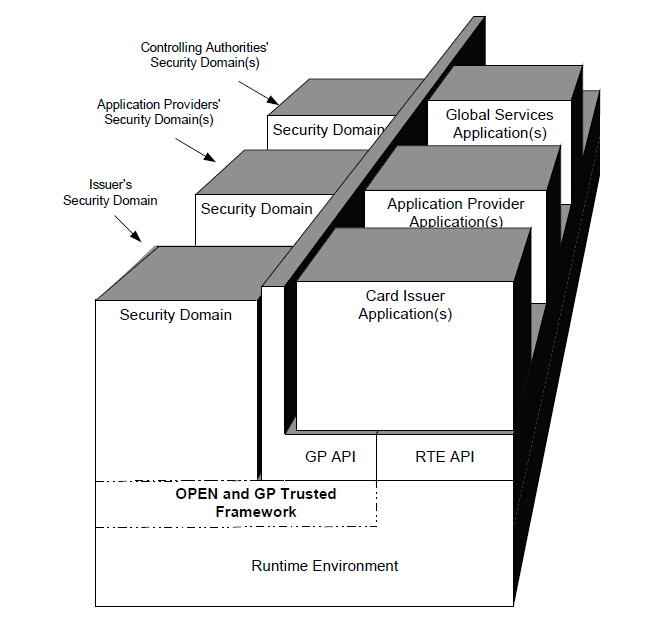
\includegraphics[width=0.7\textwidth]{gp_1.jpg}
		\caption{Card Operation System Architecture\cite{gp}}
	\label{fig:gp_1}
\end{figure}
GlobalPlatform is an international non-profit organization that provides standardized specifications for multiple smart card applications. It is now widely accepted and used as industry standard for managing Java Applet based application on Javacard Operation System in several domains, for instance in communication industries and payment company\cite{gp}. 

As shown in figure~\ref{fig:gp_1},  the GlobalPlatform card architecture contains four essential parts. The runtime environment, that provides hardware-neutral API for card application  and manages card memory spaces. The on card installed applications, which offers customers various functionalities and services. The security domain (SD), that is usually associated with particular application and known as on-card representatives  of off-card  authorities. SD is in charge of message encryption as well as decryption, creation and validation of digital signature and handling keys used in cryptographic processes. The last component is OPEN framework\cite{gp}.

\subsection{OPEN - GlobalPlatform Environment}
OPEN provides various sets of APIs offering functionalities such as entity authentication, remote data exchange, secure channel configuration and remote application management. This framework also performs APDU dispatching as well as is application selection and logical channel management\cite{gp}. Logical channel is designed to enable the data exchange between multi applications and one terminal. Each opened logical channel will handle message regard of one application.  Moreover the special logic channel named basic channel is always opened. In order to ensure system security, OPEN supports secure mechanisms such as,  user authentication , resource availability guarantee and secure channel protocol .
\paragraph{Secure Channel Protocol}
In particular, GlobalPlatform has designed the secure mechanism: secure channel protocol, to guarantee a secure communication. It ensures confidentiality of exchanged information and offers data integrity check.  Moreover Secure Channel Protocol also introduces  a cryptographic exchange process to let smart card and off-card entities to perform entity authentication with each other. 
 \begin{figure}[!htbp]
	\centering
	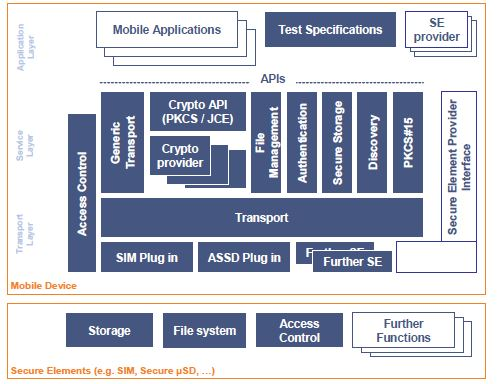
\includegraphics[width=0.8\textwidth]{open-architecture.jpg}
		\caption{OpenMobileAPI architecture overview\cite{open}}
	\label{fig:open-architecture}
\end{figure}

\section{OpenMobileAPI}
OpenMobileAPI, provided by SIMalliance, constructs an interface between terminal and chip card, which can be used by on terminal installed mobile application to access recourse stored on smart card as well as call function provided by smart card applet. Moreover OpenMobileAPI offers security mechanisms such as access control, that can be applied for mutual authentication between application and secure element. Figure~\ref{fig:open-architecture} presents an architecture overview of OpenMobileAPI, which consist of three functional layers:
 \begin{itemize}
  \item \emph{Transport Layer:} This layer is in charge of providing secure elements access control services using APDUs and acts as cornerstone for other two layers.
  \item \emph{Service Layer:} Abstract interfaces, that provide various functions such as secure storage, cryptographic services, are offered by this layer.
  \item \emph{Application Layer:} Mobile applications which benefit from OpenMobileAPI lie in this layer.
\end{itemize}

\section{Android}
\subsection{Overview}
Android is an open source platform based on Linux and modified by Google, which is designed for mobile devices. As a comprehensive platform, android manages to create a separation between hardware and software that runs on it.  At the same time being an open source project means its entire stack is open and android developers are able to deploy their androids system on any specific hardwares as well as to learn the system to the fundamental level.\cite{learn_android}
Moreover, android system provides a list of attracting software and hardware features to his customers, such as:
\begin{itemize}
\item \emph{Security:} Linux, as the cornerstone of android, has been proved to be a secure system through many harsh tests over the years. Which in return guarantees the android system security. \cite{learn_android}
\item \emph{Multi-Media:} A wide range of media formats are supported by Android. For instance: MPEG4, ACC, PNG, GIF and so on\cite{android_media}. As a result Android customers are able to enjoy a more comfortable user experiences and better entertainment functionalities.
\item \emph{Designed for Online:} One outstanding core feature of Android system is the ability to stay Online\cite{android_forensics}. Under various conditions such as Wi-Fi network, GSM/CDMA and so on, android device always provide its end users qualified network connection.
\item \emph{Variety of applications :}As one of the most popular platform,  Android, with the help of Android Market and a great number of talent Android application developers, offers its customers the possibility to extend  functionalities of their android devices\cite{android_forensics}. Android user is capable of downloading and installing various innovative applications from Android Market and enhancing the user experience.
\end{itemize}
\subsection{Android Software Stack}
\begin{figure}[!htbp]
	\centering
	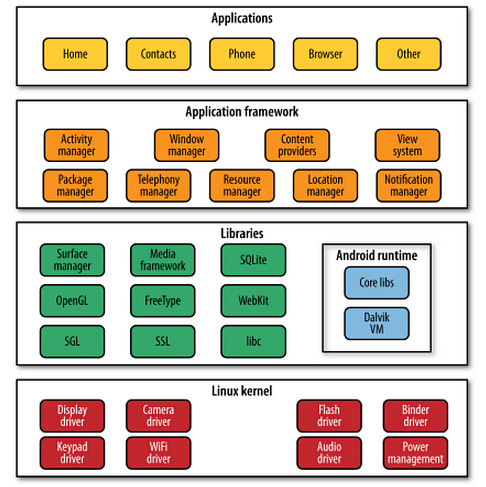
\includegraphics[width=0.85\textwidth]{android-stack.jpg}
		\caption{Android Stack Overview \cite{learn_android}}
	\label{fig:android-stack}
\end{figure}
Android stack is composed of four different layers as shown in figure~\ref{fig:android-stack}.

\subsubsection{Linux kernel:}This fundamental layer separates other three layers  from  device hardware and provides core functions such as  power and hardware driver management.
\subsubsection{Libraries:}As second layer of android stack,  Libraries layer supports android runtime environment by applying various C/C++ core libs, that offer most of the Java-functionalities.  Also in this layer, the for android specific designed virtual machine, namely Dalvik\cite{learn_android} is deployed. There exits two reasons for not using standard Java VM\cite{learn_android}. First of all, since Java VM is generally developed virtual machine, therefore some constrains from mobile systems and devices are not concerned, such as \emph{processing gap} and \emph{battery gap}\cite{embedded_secure}. Processing and battery gap refer the limited process capabilities and battery lifetime provided by mobile device. Secondly, when Android project was being carried out, Java VM didn't  belong  to the open source projects. For these reasons Dan Bornstein and his group developed the license free and mobile platform specific virtual machine, Dalvik. 

Moreover other libraries which provide services to application framework layers are also included in this Libraries layer, for instance:
\begin{itemize}
\item OpenGL, library that supports 2D and 3D graphics rendering.
\item SSL, the widely applied secure socket layer library.
\item  SQLite, which provides lightweight SQL database services.
\item  WebKit, the fast  web-rending engine.
\end{itemize}
\subsubsection{Application  framework} Application framework layer provides a large amount of application framework components, for instance activity manager which is in charge off managing application life cycles, content providers that controls data exchange between applications.
\subsubsection{Application}As the top layer of entire android software stack, application layer with the help of both native and third party reside component from application framework layer, provides various services to end users.

\subsection{Android, Dalvik and Java}
As described above, Dalvik VM compared with general Java virtual machine, takes the constrains that are specific about mobile device into account, which means this android virtual machine concerns the hardware shortcomings including less memory space, low processing power, no swap space as well as short battery lifetime. Minimum recommendations for android device\cite{android_vm} are list in table~\ref{android-min-req}.
\begin{center} 
\begin{table}[h]
\caption{Minimum Android Recommendations\cite{android_vm}}
\label{android-min-req}
\begin{tabular}{|l|l|}
\hline
Feature          & Minimum Requirement                                                                                                   \\ \hline
Chipset          & ARM-based                                                                                                             \\ \hline
Memory           & 128 MB RAM; 256 Flash External                                                                                        \\ \hline
Storage          & Mini or Micro SD                                                                                                      \\ \hline
Primary Display  & QVGA TFT LCD or larger, 16-bit color or better                                                                        \\ \hline
Navigation  keys & \begin{tabular}[c]{@{}l@{}}5-way navigation with 5 application keys, power,\\ camera and volume controls\end{tabular} \\ \hline
Camera           & 2MP CMOS                                                                                                              \\ \hline
USB              & Standard mini-B USB interface                                                                                         \\ \hline
Bluetooth        & 1.2 or 2,0                                                                                                            \\ \hline
\end{tabular}
\end{table}
\end{center}

 \begin{figure}[!htbp]
	\centering
	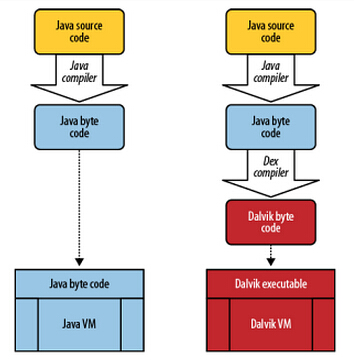
\includegraphics[width=0.55\textwidth]{vm-compare.jpg}
		\caption{Compiling process difference\cite{learn_android}}
	\label{fig:vm-compare}
\end{figure}
When Dalvik virtual machine is applied, the compiling process is different from what is taken by Java VM. Figure~\ref{fig:vm-compare} clearly pictures the difference. In Android runtime environment, after the first compilation of Java source code, the newly generated Java byte code will be compiled by Dalvik Dex complier, as a result, Dalvik byte code is created, which is going to be executed by Dalvik VM.

As pictured in figure~\ref{fig:class-vs-dex}, compared with \emph{.class} Java byte code, \emph{.dex} code adopts shared and type specific constant pools with the main purpose of conserving memory\cite{android_vm}. To be more specifically,  the constant pool in Java byte code, which is colored blue in left side of above-mentioned figure, is heterogeneous, which means all kinds of constant pools are included in this heterogeneous constant pool, even if they could be unnecessary. As a consequence, duplication may occur in Java byte code.    

Another obvious distinguish between Java VM and Delvik is that, the former one adopts stack-based architecture and  the later one uses register-based architecture, that in comparison with stack-based architecture needs on average 32.3\% less execution time\cite{android_vm}, which is obviously the better choice for the system that runs on mobile devices with limited battery life.

 \begin{figure}[!htbp]
	\centering
	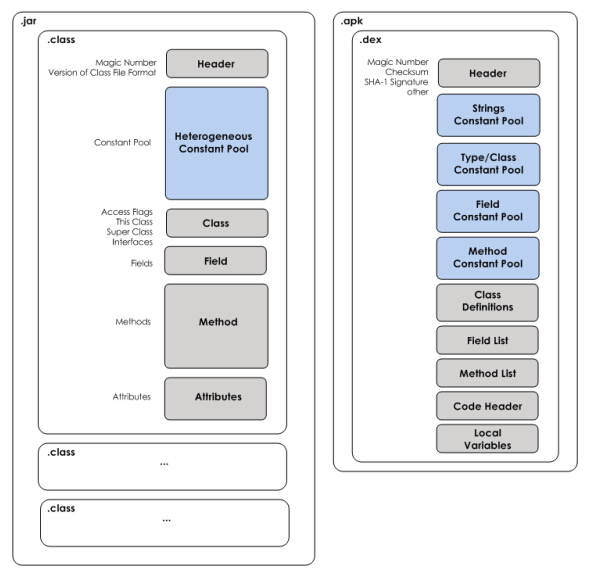
\includegraphics[width=0.85\textwidth]{clas-vs-dex.jpg}
		\caption{Comparison between Java byte code and Dalvik executable file\cite{android_vm}}
	\label{fig:class-vs-dex}
\end{figure}

\subsection{Android Application Overview} \label{secAppComponents}
One Android application consist of four components, they are activities, services, content providers and broadcast receivers\cite{android_secure_design}. Let's look into them a little deeper.
\begin{itemize}
\item  \emph{Activities} The main responsibility of android activity is provide end user an visual interface, with whose help the user can interact with the application.  
\item  \emph{Services} Services are the important components that actually provide specific functionalities to the user through the  GUI interface.
\item  \emph{Content Providers} Content Provider provides standardized and unified interfaces in order to perform shared data exchange among various applications.
\item  \emph{Broadcast Receivers} The last component is broadcast receiver, who is in charge of  asynchronously communication with android system broadcast and other applications. For example, when the battery life runs almost out, broadcast receiver will then be informed by the android OS.
\end{itemize}

\subsection{Intent} \label{secIntent}
For the purpose of inter- and intra- application communications, Android applies \emph{intent}, which is in nature a self-contained object, that includes the target application reference and alternatively the to be shared data.  Intent can be also understood as a well-formed message format that builds the Android message passing system\cite{android_secure_inter}.
